\chapter*{Remerciements}
%
Je tiens à remercier M. Fabio Pistolesi. En tant que tuteur de stage, il a su être d'un grand soutien pédagogique et moral. Je lui remercie aussi pour ses remarques constructives et critiques qui m'on permit d'améliorer mon travail et mon approche de la recherche.


J'ai également eu la chance exceptionnelle de bénéficier non pas d'un, mais de deux tuteurs de stage. Je tiens à remercier chaleureusement M. Rémi Avriller pour sa patience, disponibilité et sa bonne humeur. 
Je lui suis aussi reconnaissant de m'avoir conduit vers les meilleurs tableaux du laboratoire, que j'ai eu le plaisir d'utiliser pour étaler mes calculs à plus d'une occasion.

Je saisis cet instant pour remercier tous les chercheurs
et autres personnels du Laboratoire Ondes et Matière d'Aquitaine, ainsi que mes chères collègues stagiaires pour leur bienveillance et leur contribution à cette excellente expérience de stage.

Enfin, je tiens à adresser mes remerciements aux responsables du département Licence de m'avoir offert l'opportunité de réaliser ce stage d'excellence.
\newline
\newline
\begin{figure}[H]
    \centering
    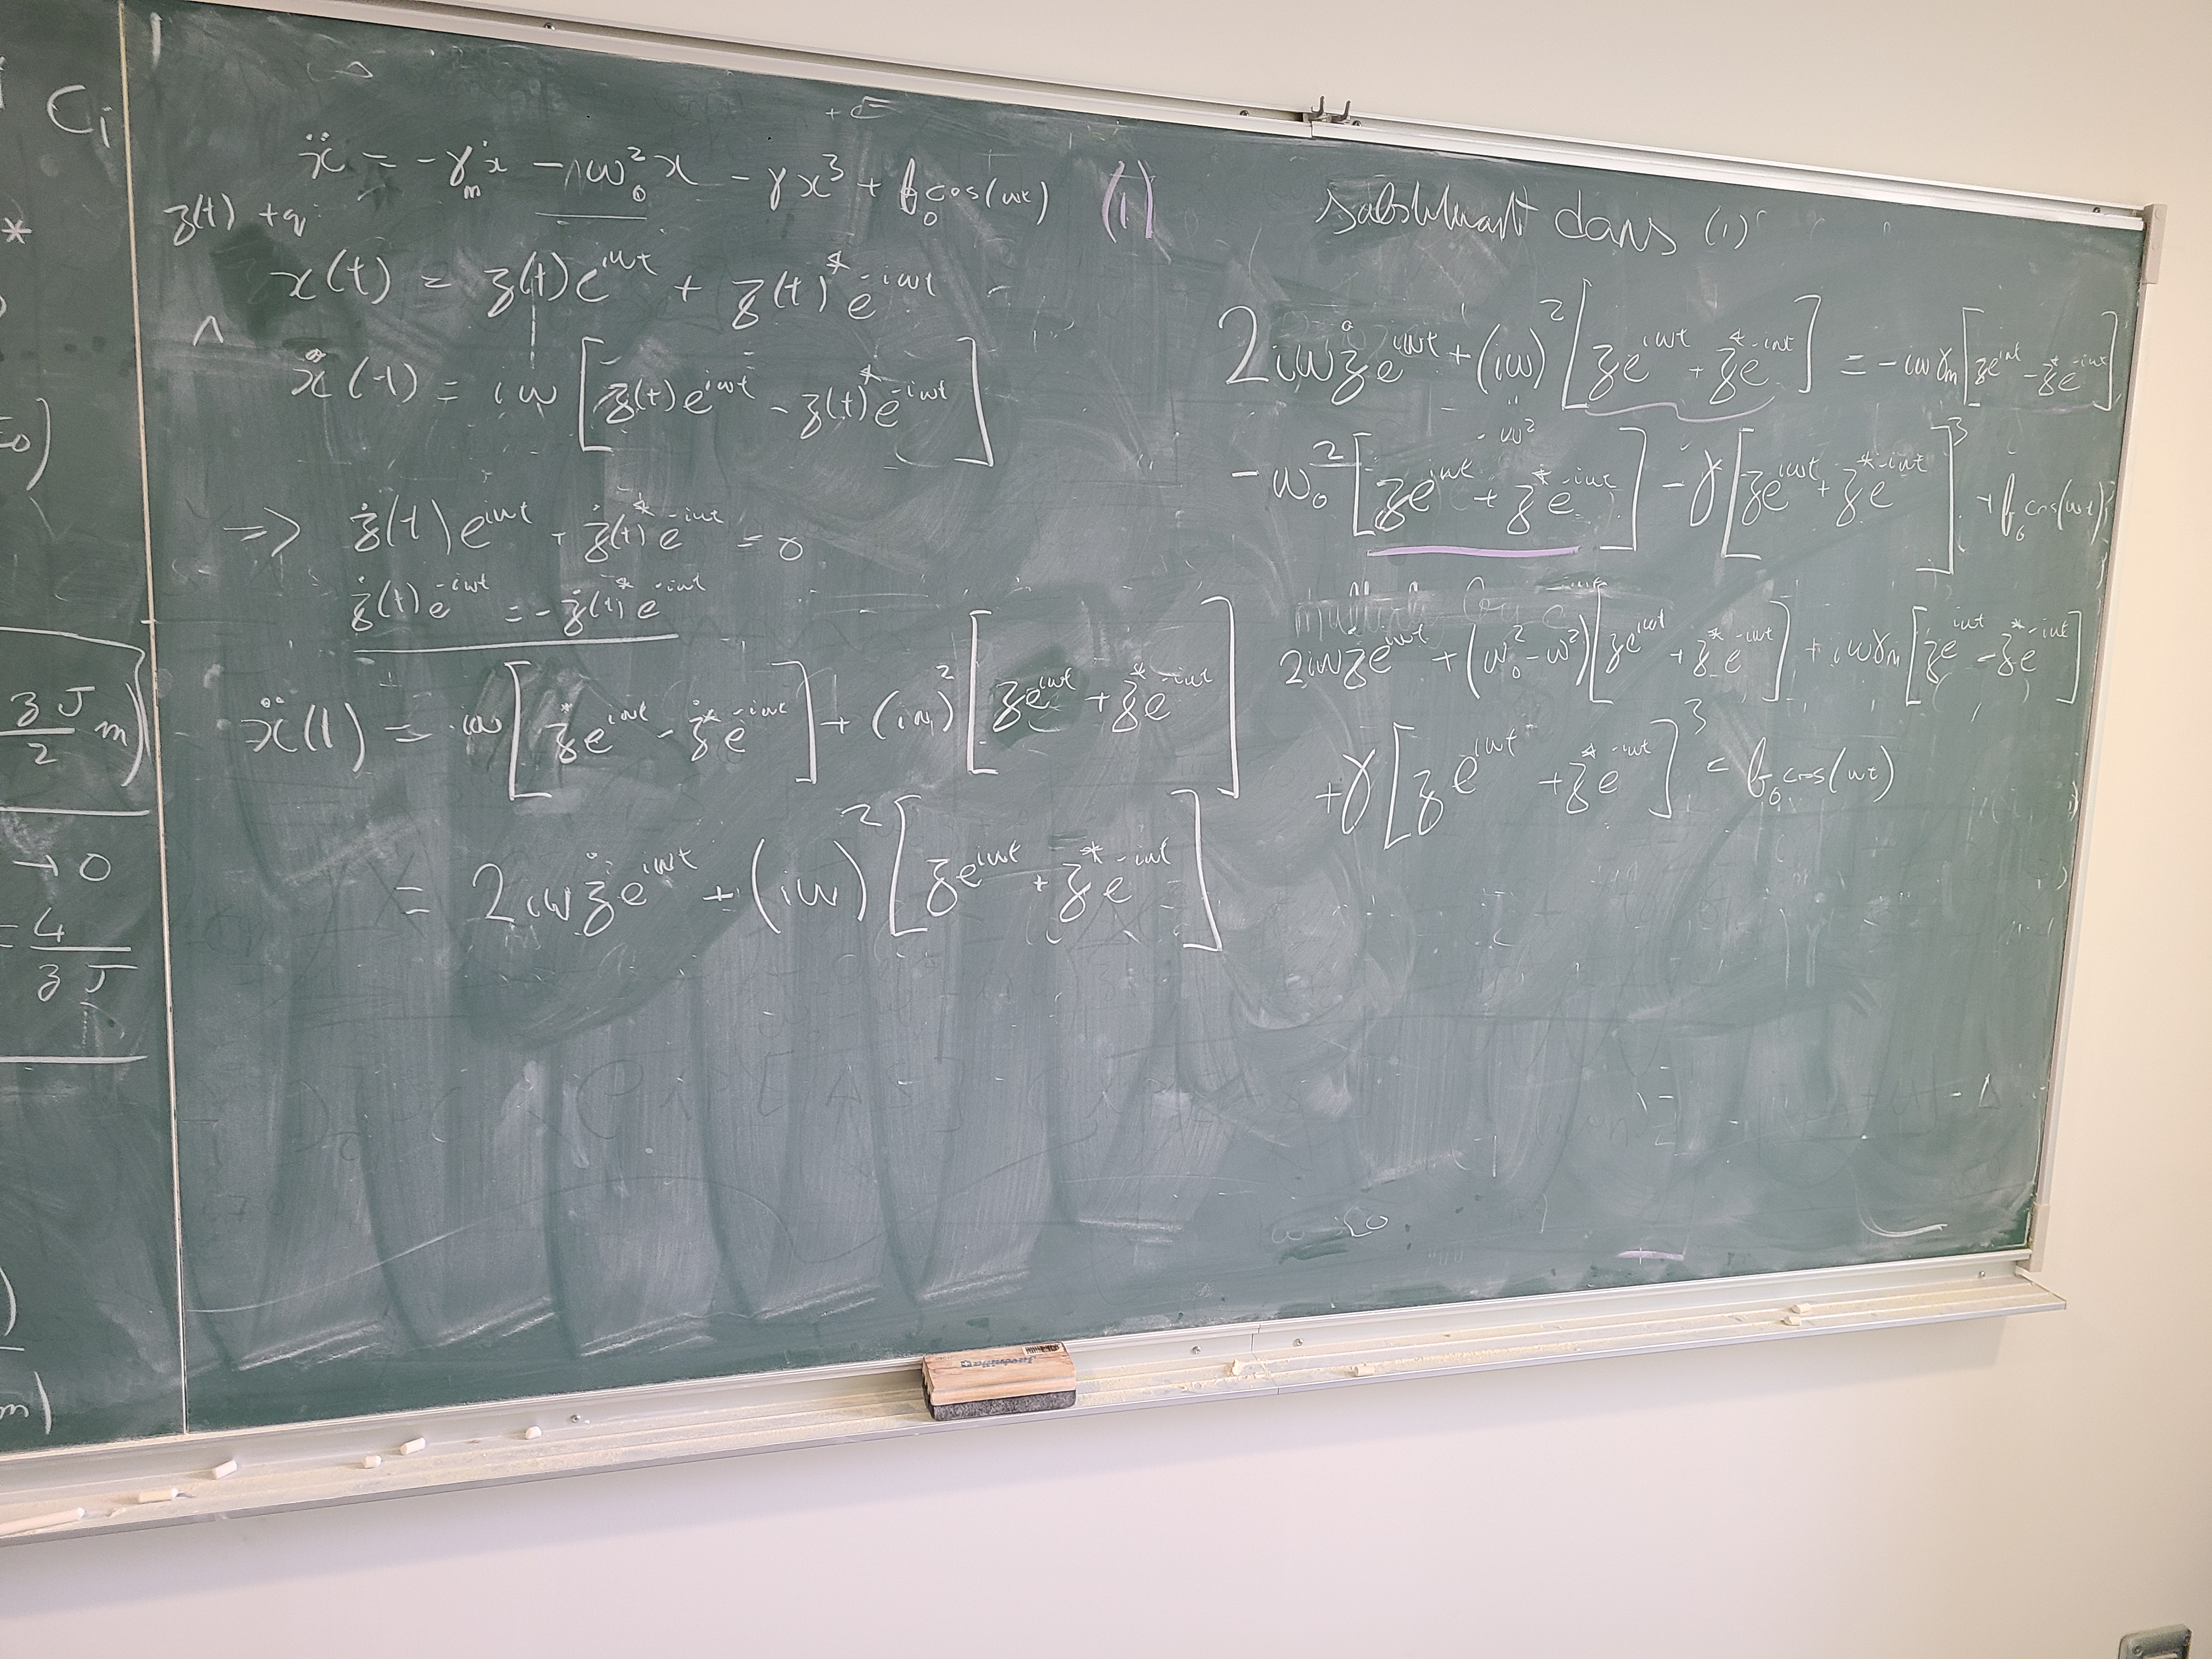
\includegraphics[width=.5\textwidth]{images/thankyou/tableux.jpg}
    \caption{Le tableau en question}
\end{figure}

